\documentclass[10pt]{article}
\usepackage{icmlko}

\icmlmeta{IP 파운데이션 월드모델}{102}{잘 붙는 축일수록 더 망친다}{노트 101의 지침을 그 지침의 방식으로 검정했더니 무작위보다 못했다 --- 상관은 진짜였고, 고른 축이 정렬에 쓰는 적재를 밀어낸 것이 원인이었다}

\begin{document}

\twocolumn[
\icmlheader

\begin{abstract}
노트 101이 지침을 세웠다 --- \textbf{긁기 전에 재라. 라벨 상관 0.2 넘는 것만
넣어라.} 그 지침 자체가 선택이므로 같은 검정을 받아야 한다. 후보 축을 스무 개
만들고(설명문 임베딩 8 · 손 특징 5 · 표지 특징 5 · 표지 주성분 2) \textbf{A반에서
상관을 재 고르고 B반에서 잰다.} 문턱을 훑었다. \textbf{단조로 나빠진다} ---
붙인 칸이 170개면 $-$0.2046, 21개면 $-$0.0316, 7개면 $-$0.0189, \textbf{0개면
$+$0.0000으로 최고}다. 그리고 \textbf{무작위보다 못하다} --- 같은 21칸을
아무렇게나 고르면 $-$0.0048인데 재서 고르면 $-$0.0316이다. \textbf{지침은
틀렸다.} 그런데 왜 틀렸는지가 뜻밖이다. \textbf{상관 자체는 진짜였다} ---
A반 $|r|$ 이 B반 $|r|$ 을 $r{=}+$0.705로 맞히고, 고른 99칸이 B반에서 상관의
81\%를 지키며 54\%가 문턱을 다시 넘는다. \textbf{실패는 통계가 아니라 기하다.}
고른 축을 넣으면 \textbf{프로크루스테스가 정렬에 쓰는 공통 축 적재가 밀려난다}
--- 모바일은 공통 블록 몫이 0.716에서 0.343으로, 팝업은 0.587에서 0.288로
준다. 붙인 축 수와 몫 감소의 상관이 $r{=}-$0.787이다. \textbf{라벨에 잘 붙는
축일수록 주성분을 자기 쪽으로 더 세게 끌어당기고, 그만큼 정렬 재료를 더 많이
밀어낸다.} 노트 36이 예견하고 꺼 둔 \texttt{block\_norm} 을 켜면 손실의 56\%가
돌아오지만($-$0.0302 $\to-$0.0134) 부호는 안 바뀐다. \textbf{덤으로 나쁜 소식
하나} --- 노트 100의 $+$0.0127도 반쪽에서는 $-$0.0045다.
\end{abstract}
]

\begin{figure*}[t]
\centering
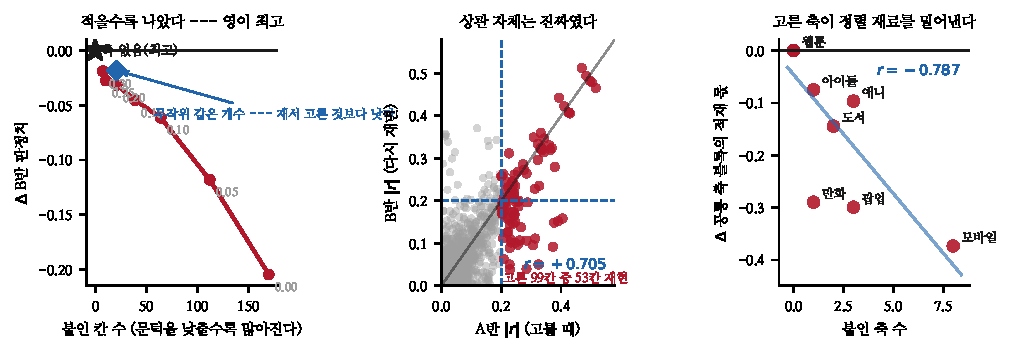
\includegraphics[width=\textwidth]{figs/cr.pdf}
\caption{왼쪽 --- 적을수록 나았다. 가운데 --- 상관 자체는 진짜였다.
오른쪽 --- 고른 축이 정렬 재료를 밀어낸다.}
\end{figure*}

\section{지침을 그 지침의 방식으로 검정한다}

후보 축을 스무 개 만들었다 --- 설명문 임베딩 $c_0\!\sim\!c_7$ · 손 특징 다섯
(길이 · 문장 수 · 문장 길이 · 어휘 다양성 · 숫자 비율) · 표지 특징 다섯 ·
표지 주성분 둘. 도메인 열과 곱해 \textbf{173칸}이고 그중 라벨 상관이 0.2를
넘는 것이 18칸이다.

\begin{table}[t]
\centering\tsize
\caption{$|$라벨 상관$|$ 상위. 전체 자료.}
\begin{tabular}{lrl}
\toprule
& $|r|$ & \\
\midrule
모바일 · emb2 & 0.490 & \\
모바일 · emb1 & 0.417 & \\
모바일 · emb5 & 0.346 & \\
\textbf{팝업 · 문장 수} & \textbf{0.312} & 기획 개념문 \\
\textbf{팝업 · 길이} & \textbf{0.283} & 기획 개념문 \\
애니 · 문장 수 & 0.240 & \\
만화 · 숫자 비율 & 0.233 & \\
아이돌 · 표지 pc1 & 0.210 & \\
\bottomrule
\end{tabular}
\end{table}

\section{단조로 나빠진다}

\begin{table}[t]
\centering\tsize
\caption{A반에서 문턱으로 고르고 B반에서 잰다. 분할 다섯 평균.}
\begin{tabular}{lrrr}
\toprule
문턱 & 붙인 칸 & B반 $\rho$ & $\Delta$ \\
\midrule
0.00 & 170.2 & $+$0.2082 & $-$0.2046 \\
0.05 & 112.2 & $+$0.2947 & $-$0.1181 \\
0.10 & 64.2 & $+$0.3514 & $-$0.0614 \\
0.15 & 39.0 & $+$0.3676 & $-$0.0453 \\
0.20 & 21.0 & $+$0.3813 & $-$0.0316 \\
0.25 & 10.4 & $+$0.3854 & $-$0.0274 \\
0.30 & 7.4 & $+$0.3939 & $-$0.0189 \\
\textbf{없음} & \textbf{0} & \textbf{$+$0.4128} & \textbf{$+$0.0000} \\
\midrule
\textbf{무작위 21칸} & 21 & $+$0.3945 & \textbf{$-$0.0183} \\
\bottomrule
\end{tabular}
\end{table}

\claimx{노트 101의 지침은 \textbf{틀렸다.} 반쪽 검정에서 문턱을 낮출수록 단조로
나빠지고 아무것도 안 붙이는 것이 최고다. 게다가 \textbf{재서 고른 21칸이
무작위 21칸보다 나쁘다}($-$0.0316 대 $-$0.0183).}{반쪽 검정은 도메인마다
레코드를 절반으로 줄인다. 팝업이 37건이 되므로 어떤 축이든 불리한 규약이다 ---
그래도 무작위와의 비교는 같은 조건이라 유효하다.}

\begin{table}[t]
\centering\tsize
\caption{같은 다섯 반쪽에서 처방을 나란히.}
\begin{tabular}{lrr}
\toprule
& B반 $\rho$ & $\Delta$ \\
\midrule
\textbf{축 없음} & \textbf{$+$0.4128} & \textbf{$+$0.0000} \\
박은 처방(emb0 · $k{=}3$) & $+$0.4084 & $-$0.0045 \\
무작위 같은 개수 & $+$0.4080 & $-$0.0048 \\
고른 처방 $\theta{=}0.30$ & $+$0.3939 & $-$0.0189 \\
고른 처방 $\theta{=}0.20$ & $+$0.3813 & $-$0.0316 \\
\bottomrule
\end{tabular}
\end{table}

\claimx{노트 100의 $+$0.0127은 \textbf{반쪽에서 재현되지 않는다} --- 같은
처방이 B반에서 $-$0.0045다. 그 수치는 아직 전체 자료 전용이다.}{반쪽은
표본이 절반이라 인자 공간이 얇아진다. 재현 실패가 ``효과가 없다''는 뜻은
아니고 ``이 규약으로는 못 본다''는 뜻이다.}

\section{상관 자체는 진짜였다}

지침이 틀렸다면 상관이 잡음이었어야 자연스럽다. \textbf{아니었다.}

\begin{table}[t]
\centering\tsize
\caption{A반 $|r|$ 과 B반 $|r|$. 824칸(분할 다섯).}
\begin{tabular}{lr}
\toprule
두 반쪽 $|r|$ 의 상관 & \textbf{$+$0.705} \\
A반 0.20 넘은 칸 & 99개 \\
\quad B반에서도 0.20 넘는 것 & 53개 (\textbf{54\%}) \\
\quad B반 $|r|$ 평균 & 0.229 (A반 0.284) \\
\quad 줄어든 몫 & 19\% \\
A반 0.20 아래 칸의 B반 $|r|$ & 0.081 \\
\bottomrule
\end{tabular}
\end{table}

\claimx{선별은 \textbf{제 일을 했다.} 고른 칸이 다른 반쪽에서 상관의 81\%를
지키고 절반 넘게 문턱을 다시 넘는다. \textbf{실패는 통계가 아니다.}}
{54\%는 절반이다. 문턱 근처 칸은 어차피 반은 떨어지므로 재현률 자체는
문턱값의 성질이기도 하다.}

\section{실패는 기하였다}

\begin{table}[t]
\centering\tsize
\caption{프로크루스테스가 쓰는 \textbf{공통 축 블록}이 상위 성분 적재에서
차지하는 몫.}
\begin{tabular}{lrrr}
\toprule
& 붙인 축 & 현행 & 붙인 뒤 \\
\midrule
\textbf{모바일} & 8 & 0.716 & \textbf{0.343} \\
\textbf{팝업} & 3 & 0.587 & \textbf{0.288} \\
\textbf{만화} & 1 & 0.920 & \textbf{0.630} \\
도서 & 2 & 0.747 & 0.602 \\
애니 & 3 & 0.472 & 0.376 \\
아이돌 & 1 & 0.567 & 0.492 \\
웹툰 · 펀딩 · 게임 · 세계애니 & 0 & --- & 변화 없음 \\
\midrule
\multicolumn{3}{l}{붙인 축 수와 몫 감소의 상관} & \textbf{$-$0.787} \\
\bottomrule
\end{tabular}
\end{table}

\claimx{고른 축이 \textbf{정렬 재료를 밀어낸다.} 프로크루스테스는 공통 축
적재만 보고 회전을 정하는데, 고유 축을 넣으면 주성분이 그쪽으로 끌려가 공통
블록의 적재 몫이 준다. 모바일 0.716$\to$0.343, 팝업 0.587$\to$0.288.
\textbf{라벨에 잘 붙는 축일수록 주성분을 더 세게 끌어당기므로 더 많이
밀어낸다} --- 지침이 고르는 것이 정확히 그런 축이다.}{몫과 성적을 직접
연결하진 않았다. 축 수와 몫 감소($r{=}-$0.787), 축 수와 성적 악화(문턱 곡선)를
따로 봤을 뿐이다.}

\begin{quote}\fontsize{9.5}{11.5}\selectfont
이것은 새 발견이 아니라 \textbf{예견의 확인}이다. \texttt{factor\_space} 의
주석이 노트 36에서 이렇게 적혀 있었다 --- ``고유 축이 다섯 개면 블록 분산이
공유 블록을 압도해 주성분이 고유 축 쪽으로 끌려가고, 정렬에 쓰는 공통 축
적재가 희석된다.'' 열여섯 노트 뒤에 그 문장이 지침 하나를 죽였다.
\end{quote}

\section{처방은 절반만 듣는다}

노트 36은 이 문제를 위해 \texttt{block\_norm} 을 만들고 \textbf{꺼 뒀다}
(당시 다섯 축 구조에서 미세하게 나빴다). 켜 봤다.

\begin{table}[t]
\centering\tsize
\caption{전체 자료. \texttt{block\_norm} 켜기.}
\begin{tabular}{lrr}
\toprule
& $\rho$ & $\Delta$ \\
\midrule
축 없음 & $+$0.4038 & --- \\
고른 처방 $\theta{=}0.20$ & $+$0.3736 & $-$0.0302 \\
\quad $+$ \texttt{block\_norm} & $+$0.3904 & \textbf{$-$0.0134} \\
박은 처방(emb0 · $k{=}3$) & $+$0.4165 & $+$0.0127 \\
\quad $+$ \texttt{block\_norm} & $+$0.4032 & $-$0.0006 \\
\bottomrule
\end{tabular}
\end{table}

\claimx{\texttt{block\_norm} 은 고른 처방의 손실을 \textbf{56\% 회복}시키지만
부호를 못 바꾼다. 그리고 박은 처방은 오히려 망친다($+$0.0127 $\to-$0.0006) ---
축이 하나뿐일 때는 밀어낼 것이 적어 보정이 과하다.}{켜고 끄는 이지선다를
설정마다 고르면 그것이 또 선택이다. 여기서는 관측만 적는다.}

\section{한계}

\begin{itemize}[leftmargin=1.1em,itemsep=0.15em]
\item \textbf{채택할 것이 없다.} 이 노트의 모든 설정이 축 없음보다 나쁘다.
\item 반쪽 검정이 표본을 절반으로 줄여 팝업이 37건이 된다. 규약 자체가
      가혹하다.
\item 적재 몫과 성적을 직접 회귀로 잇지 않았다.
\item 후보 축 스무 개가 전부 설명문 · 표지에서 나온 것이다. 다른 종류의
      축은 다르게 행동할 수 있다.
\item 노트 101의 $r{=}+$0.695는 살아 있다(애니 · 모바일을 빼도 $+$0.543).
      \textbf{같은 축을 여러 도메인에 붙일 때}의 법칙과 \textbf{여러 축 중
      고를 때}의 법칙이 다르다는 것이 이 노트의 정정이다.
\end{itemize}

\section{다음}

\begin{enumerate}[leftmargin=1.3em,itemsep=0.15em]
\item \textbf{정렬을 안 쓰는 길} --- 밀어냄이 프로크루스테스 때문이라면
      정렬이 필요 없는 구조에서는 안 생겨야 한다. 노트 93의 직접 전이를
      새 축과 함께 다시 본다.
\item \textbf{공통 축을 늘린다} --- 밀어냄은 공통 블록이 다섯뿐이라 생긴다.
      새 축을 \emph{고유}가 아니라 \emph{공통} 슬롯으로 넣을 수 있는지 본다.
      도메인 여럿이 같은 축을 가지면 가능하다(설명문은 아홉이 갖는다).
\item \texttt{block\_norm} 을 규칙으로 고정한다 --- ``고유 축이 둘 이상이면
      켠다'' 같은 미리 박은 규칙으로. 고르는 것이 아니어야 한다.
\item 반쪽 검정 대신 \textbf{시간 분할}(노트 77)로 판정한다. 표본을 안 줄인다.
\end{enumerate}

\vspace{0.6em}
\hrule height 0.3pt
\vspace{0.5em}
{\footnotesize
\textbf{참고문헌}\\[0.3em]
Schoenemann, P. H. (1966). A generalized solution of the orthogonal Procrustes
problem. \emph{Psychometrika}, 31(1), 1--10.\\[0.15em]
Guyon, I., Elisseeff, A. (2003). An introduction to variable and feature
selection. \emph{JMLR}, 3, 1157--1182.\\[0.15em]
Cawley, G. C., Talbot, N. L. C. (2010). On over-fitting in model selection and
subsequent selection bias in performance evaluation. \emph{JMLR}, 11, 2079--2107.\\[0.15em]
Meredith, W. (1993). Measurement invariance, factor analysis and factorial
invariance. \emph{Psychometrika}, 58(4), 525--543.\\[0.15em]
Ben-David, S. et al. (2010). A theory of learning from different domains.
\emph{Machine Learning}, 79(1--2), 151--175.
}

\end{document}
